\chapter{Predictive Analytics im öffentlichen Sektor}

Die Methode des Forecasting hat (bisher) noch keinen bedeutenden Durchbruch in
der breiten Öffentlichkeit gehabt\footnote{

}. Es gibt Stimmen, die behaupten, dass ein immenser Widerstand gegen die
Einführung dieser Methode zu erwarten ist. Teilweise deutet sich sogar eine
Unmöglichkeit dieser Aufgabe an. 
Beim Thema Forecasting ist es Tetlock selbst, der sich skeptisch äußert. Er
benennt den Widerstand der Experten als die größte Barriere zur Einführung der
neuen Methodik (\emph{the most daunting of all the barriers to implementation},
vgl. \cite{Tetlock}, S.~235). Jackson und Reichin vertreten eine ähnliche
Auffassung (vgl. \cite{Jackson}, S.~295). 

Für Predictive Analytics sind die Prognosen optimistischer (vgl. \cite{Mauerer}).
Allerdings ist zweifelhaft, ob Top Manager \emph{ihre} Entscheidungen mit Hilfe
von Predictive Analytics Methoden treffen.
Unternehmen behaupten zwar, dass strategische Entscheidungen mit Hilfe von Predictive Analytics
unterstützt werden sollen (vgl. \cite{Mauerer}, S.~2), die konkreten Anwendungsbeispiele deuten
aber darauf hin, dass hauptsächlich operative Abteilungen (wie z. B. der Kauf und Verkauf von
Gütern) betroffen sind.

Somit deutet sich die Frage an, ob grundsätzliche Hindernisse bestehen, die verhindern, dass sich
evidenzbasierte Methoden wie Forecasting und Predictive Analytics auf allen Ebenen der
Entscheidungshierarchie etablieren. Diese Fragestellung wird im folgenden Text untersucht werden.

\section{Rahmenbedingungen}

Bei der folgenden Analyse ist es sinnvoll zwischen strategischer, taktischer und
operativer Ebene zu unterscheiden. Im Allgemeinen lassen sich die verschiedenen
Ebenen wie folgt abgrenzen:

\begin{description}

\item[Strategische Ebene:] \hfill \\
Bei der strategischen Ausrichtung einer Organisation werden allgemeine, wegweisende Ziele definiert
und es werden den Zielen Prioritäten zugewiesen. Strategische Entscheidungen werden in 
der Regel vom Top Management gefällt. Im öffentlichen Sektor sind führende Politiker, 
wie beispielsweise Minister, und hohe Staatsbeamte die Entscheidungsträger auf dieser Ebene.
Die politische Weltanschauung der Entscheidungsträger hat auf dieser Ebene den 
meisten Einfluss auf die gewählten Ziele und ihre Prioritäten.

\item[Taktische Ebene:] \hfill \\
Die Aufgabe der taktischen Ebene ist die Entwicklung eines Vorgehens, das es
ermöglicht, die strategischen Ziele der Organisation zu erreichen. Die strategischen
Prioritäten sollten dabei, wenn möglich, ebenfalls eingehalten werden. Entscheidungen
auf der taktischen Ebene werden vom mittleren Management und seltener auch vom Top
Management getroffen. Staatsbeamte im mittleren und gehobenen Dienst, sowie Projektmanager von
Unternehmen, die öffentliche Aufträge bearbeiten, sind die Entscheidungsträger auf der taktischen
Ebene im öffentlichen Sektor. Die politische Weltanschauung der Entscheidungsträger hat 
auf die taktische Ebene weniger Einfluss als auf die strategische Ebene. 

\item[Operative Ebene:] \hfill \\
Entscheidungsträger auf der operativen Ebene haben die Aufgabe das \glqq{Tagesgeschäft}\grqq{}
zu überwachen und sicherzustellen, dass die Vorgaben der taktischen Ebene eingehalten werden.
Das operative Management und auch Angestellte ohne besondere Führungsaufgaben treffen operative
Entscheidungen, wobei ihr Spielraum dabei durch die Entscheidungen der strategischen und taktischen
Ebene meist stark eingeschränkt ist. Im öffentlichen Sektor führen Beamte im mittleren Dienst und 
operative Manager von Firmen mit öffentlichen Auftraggebern Tätigkeiten auf operativer Ebene aus.

\end{description}

Weiterhin wird nicht davon ausgegangen, dass wichtige taktische und strategische Entscheidungen
vollkommen automatisiert getroffen werden können. Vielmehr wird im besten Fall ein Zusammenspiel
erwartet, bei dem Menschen entscheiden und Computer sie dabei unterstützen.



% TODO Technologie prinzipiell kein Hindernis (s. IT Novum)

% TODO
% Stand Entscheidungshilfen (wie vorstellbar: Mensch entscheidet, Computer
%   unterstützt)
% Abgrenzung zum privaten Sektor
% auf operativer Ebene allerdings ähnlich
% unterschied strategisch, taktische Ebene, operativ
 
% s. Watson, Abschnitt Lack of regulation and algorithm bias

\begin{figure}%[!hbt]
\centering
\caption{Risikomatrix für die Nutzung maschineller Entscheidungshilfen}
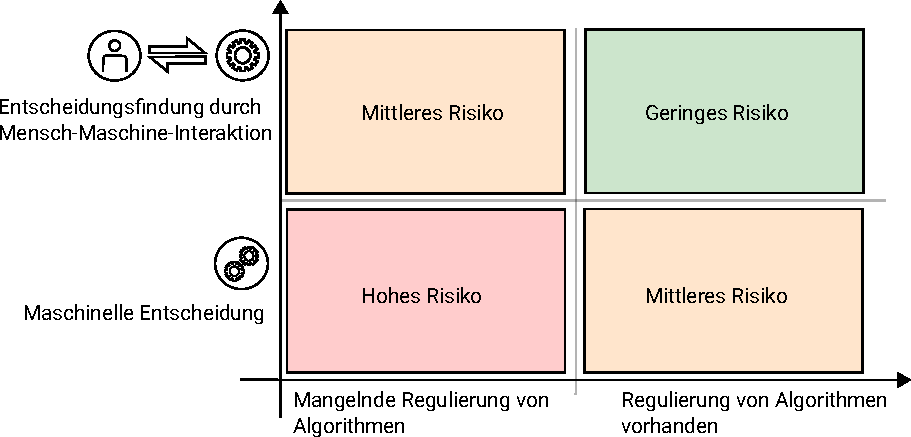
\includegraphics[scale=1.0]{Grafiken/Risk_Matrix_Ink.pdf} 
\label{pic:Risiko_Matrix}
\end{figure}





% TODO
% Politiker, Experten und Kommentatoren formulieren keine subjektiven Wsk und
% niemand berechnet den Brier Score (oder ein anderes Maß)
% 


%-------------------------------------------------------------------------------
% Tetlock kam bei seiner Studie zu dem Urteil, ...
Tetlock ist der Meinung, dass die Kernaufgabe politischer Weltanschauungen
nicht die Erstellung möglichst korrekter Prognosen ist, sondern die
Aufrechterhaltung einer bequemen Illusion von Berechenbarkeit
(vgl. \cite{Tetlock}, S.~39). Somit sind die Ergebnisse schlecht, weil keine
genaue Abbildung der Realität beabsichtigt wird. Die Aufrechterhaltung von
Glaubenssätzen, die zum kollektiven Zusammenhalt beitragen, hat höhere
Priorität.

In diesem Zusammenhang sind auch verschiedene Interpretationen des
Wahrheitsbegriffs bedeutsam. Eine weit verbreitete Interpretation wird mit
Hilfe des Pragmatismus von William James definiert (vgl. \cite{Precht}). Demnach werden
Aussagen von Menschen als Wahrheit akzeptiert, falls die Aussagen ihnen bei der
Orientierung in der Welt nützlich sind. Dies liefert eine Erklärung dafür, dass
Menschen dazu tendieren Aussagen zu glauben, die ihre eigene Weltsicht
bestätigen. Bei einer extremen Ausprägung des pragmatischen Wahrheitsbegriffs
wird aus der Nützlichkeit einer Aussage ihr Wahrheitsgehalt abgeleitet:
\glqq{Es ist wahr, weil es nützlich ist}\grqq.

Diese radikale Wahrheitsinterpretation ist problematisch, wenn die als Wahrheit
betrachteten Grundsätze der Realität widersprechen. Denn es gibt keine
Möglichkeit, die Grundsätze mit Hilfe von empirischen oder logischen Beweisen
zu revidieren und an die Realität anzupassen. Langfristig führen falsche
Grundsätze somit zu schlechtem Urteilsvermögen, was wiederum zu schlechten
Entscheidungen führt. Insbesondere sind Datenanalysen in einer solchen Situation
nicht zweckdienlich, da Ergebnisse selektiv ignoriert oder abgelehnt werden.

Eine andere Interpretation von Wahrheit legt großen Wert auf die Beweisbarkeit
von Aussagen. Eine solche Interpretation ist beispielsweise in der Wissenschaft
verbreitet. Aussagen wird erst dann ein Wahrheitswert zugewiesen, wenn
unwiderlegbare Beweise für die Gültigkeit der Aussage vorhanden sind. Eine
solche Interpretation weicht stark vom pragmatischen Standpunkt ab, kann aber
ebenfalls problematisch werden. Es besteht die Gefahr sich bei der Prüfung von
Aussagen in Kleinigkeiten zu verlieren, handlungsunfähig zu werden oder
nützliche Erkenntnisse zu lange anzuzweifeln\footnote{
Beispiele für Zweifel, die gefährlich werden, weil sie Fortschritt blockieren
sind auf Seite~\xcom erläutert.
}.

Vermutlich ist für ein gutes Urteilsvermögen ein nüchterner Pragmatismus
notwendig, bei dem vorsichtig zwischen Nutzen und Wahrheit abgewogen wird und
auch unangenehme Meinungen als Wahrheit akzeptiert werden können.
Bedauerlicherweise gerät ein solcher Pragmatismus mit jeder, insbesondere
politischen, Weltanschauung in Konflikt, die selbst nicht in ähnlicher Weise
pragmatisch ist.

%-------------------------------------------------------------------------------

\subsection{Eine pessimistische Sichtweise}

%\subsubsection{}

% TODO

% 3 Ängste: Verlust Privilegien, Verlust der Arbeit, Verlust der (kollektiven) Identität

%Je mehr das Treffen von Entscheidungen zur Hauptaufgabe von Personen gehört,
%desto stärker betrachten sie \emph{predictive analytics} als eine Gefahr für
%ihren Arbeitsplatz.

%Zudem spielen politische Faktoren im öffentlichen Sektor eine größere Rolle als
%im privaten Sektor.

%Es ist zu erwarten, dass sich Predictive Analytics am leichtesten auf der operativen Ebene etablieren
%lässt, da das Führungspersonal der taktischen und strategischen Ebene über mehr Macht verfügt.

% - versch. Gruppen/Kulturen -> versch. Wahrheiten

% Forecasting leichter zu sehen,
% 
% 
% - Wahrheit taktisch genutzt

% - Themen kontroverser (vs. z. B. Fruchtsäfte)
% - 
% - Ignorieren (-> Probleme menschl. Urteile)

%Der investigative Charakter von Datenanalysen kann Nervosität und Unbehagen
%auslösen.


\subsection{Eine optimistische Sichtweise}

% + MÖGLICHKEIT BESSERE ENTSCHEIDUNGEN ZU TREFFEN

% Formalisierung erwünscht (BBC + IC)

% 

Bessere Prognosen und Urteile führen zu besseren Entscheidungen. Dies bringt
wiederum sowohl Vorteile gegenüber Konkurrenten als auch Vorteile bei der
Auseinandersetzung mit der \glqq{Natur}\grqq\footnote{
Genauer: Bei der Auseinandersetzung mit den Zwängen, die durch die Naturgesetze
und ökonomische Prinzipien definiert werden. Verzichtet man zum Beispiel auf das 
Rauchen kann es als eine gute Entscheidung betrachtet werden, da man dadurch
gesünder lebt. Hierfür muss zunächst erkannt werden, dass Rauchen ungesund ist.
Klingt heute einfach. Diese Erkenntnis zu erlangen war jedoch mit erheblichem
Aufwand verbunden, wobei auch wissenschaftliche und statistische Methoden
eine große Rolle spielten (vgl. zum Beispiel \cite{Proctor}).

Ein weiteres Beispiel für eine Entscheidung, die nicht in erster Linie Vorteile
gegenüber Konkurrenten verspricht, ist eine Entscheidung für eine bessere
Behandlungsmethode in der Medizin. Denn der primäre Zweck davon ist, 
mehr Menschen eine Heilung zu ermöglichen.
}

\section{Spieltheoretische Betrachtung}

Aufgrund der potentiell konfliktreichen Situation rund um die Einführung von
\emph{forecasting} oder \emph{predictive analytics}, bietet es sich an, die
\gls{glos:Spieltheorie} anzuwenden.

\subsection{Einleitung zur Spieltheorie}
% TODO


% deadlock (S. 218(
\begin{figure}%[!hbt]
\centering
\caption{Deadlock Auszahlungsmatrix}
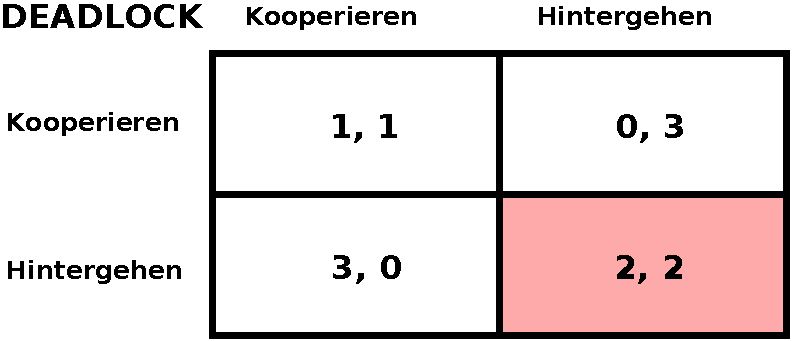
\includegraphics[scale=0.8]{Grafiken/Deadlock_Ink.pdf} 
\label{pic:Deadlock}
\end{figure}

% stag hunt (S. 220)
\begin{figure}%[!hbt]
\centering
\caption{Stag Hunt Auszahlungsmatrix}
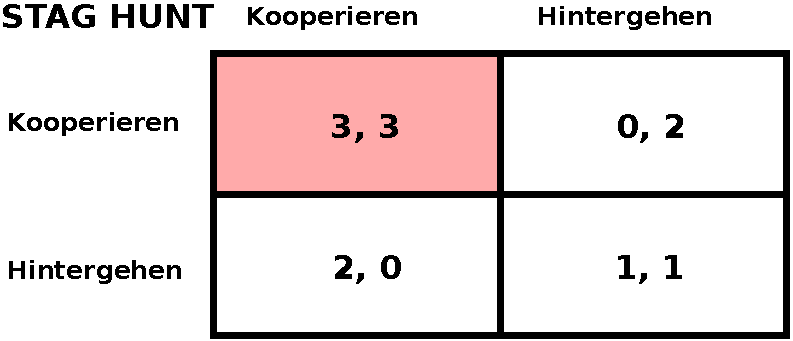
\includegraphics[scale=0.8]{Grafiken/Stag_Hunt_Ink.pdf} 
\label{pic:StagHunt}
\end{figure}

% mixed
\begin{figure}%[!hbt]
\centering
\caption{Gemischte 'Stag Hunt - Deadlock' Auszahlungsmatrix}
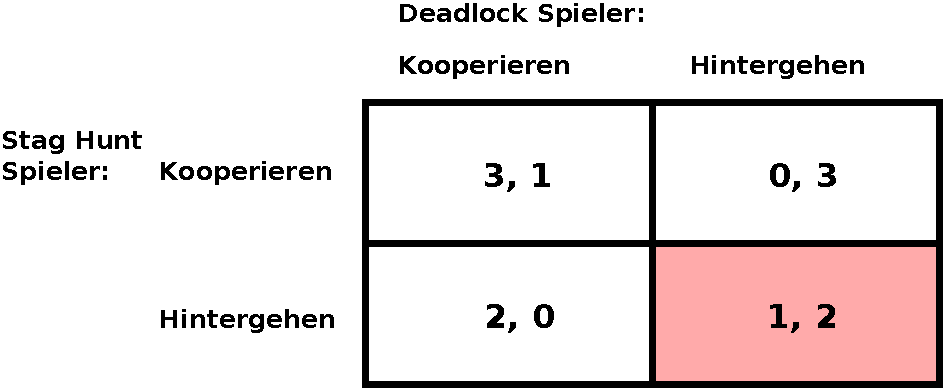
\includegraphics[scale=0.7]{Grafiken/Mixed_Ink.pdf} 
\label{pic:Mixed}
\end{figure}

\subsection{Kritische Würdigung der spieltheoretischen Betrachtung}

% TODO spielen implizit spieltheorie (s. Poundstone ?)

% prisoners dilemma (S.237)
% mixed
\begin{figure}%[!hbt]
\centering
\caption{Gefangenendilemma Auszahlungsmatrix}
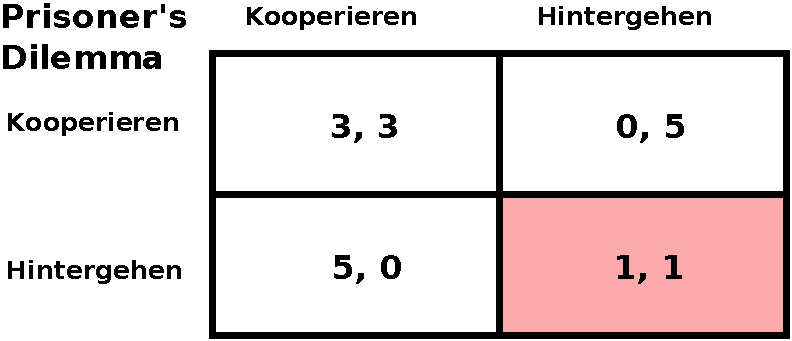
\includegraphics[scale=0.8]{Grafiken/Prisoner_Ink.pdf} 
\label{pic:Prisoner}
\end{figure}